\chapter{Segmentação}

Para selecionar um determinado tipo de tecido da imagem, é utilizado o recurso de 
segmentação, disponível no InVesalius.

\section{Limiar (\textit{Threshold})}

Limiar é uma técnica de segmentação de imagens que permite selecionar da imagem somente
os \textit{pixels} cuja intensidade está dentro de um limiar definido pelo usuário.
O limiar é definido por dois números, limiares inicial e final, também conhecidos como
\textit{thresholds} mínimo e máximo. Como referência para a definição, é utilizada a
escala de Hounsfield (tabela \ref{tab:escala_hounsfield}).

A segmentação é acionada no painel situado no lado esquerdo da interface do InVesalius,
no item \textbf{2. Selecione a região de interesse} (figura \ref{fig:region_selection}).

\begin{figure}[!htb]
\centering
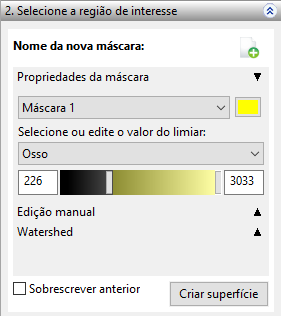
\includegraphics[scale=0.6]{../user_guide_figures/invesalius_screen/segmentation_threshold_window_left_pt.png}
\caption{Seleção de região de interesse}
\label{fig:region_selection}
\end{figure}

Antes de iniciar a segmentação, é necessário configurar uma máscara. A máscara é uma
imagem com a região selecionada colorida e sobreposta à imagem original. Veja a figura
(\ref{fig:region_selection_masc})

\begin{figure}[!htb]
\centering
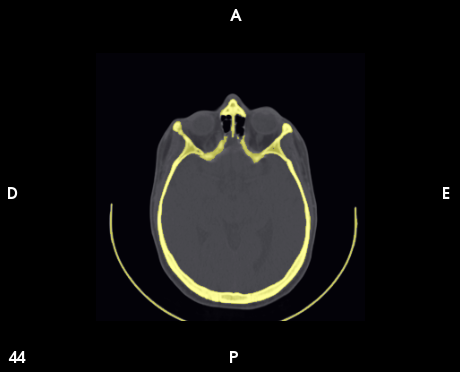
\includegraphics[scale=0.4]{../user_guide_figures/invesalius_screen/segmentation_threshold_axial_pt.png}
\caption{Máscara (regiões em amarelo)}
\label{fig:region_selection_masc}
\end{figure}

Para alterar o limiar, pode-se utilizar a barra que representa os níveis de cinza na imagem (figura
\ref{fig:region_selection_bar}). É possível alterar o limiar inicial usando o controle deslizante
\textit{esquerdo} da barra. De forma semelhante, o limiar final pode ser alterado por meio do controle
\textit{direito}. É possível, ainda, digitar diretamente os valores desejados nas respectivas caixas
de texto nas extremidades da barra. Com a alteração dos valores, automaticamente a máscara será atualizada,
pintando somente os \textit{pixels} com intensidade dentro da faixa determinada.

\begin{figure}[!htb]
\centering
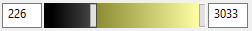
\includegraphics[scale=0.75]{../user_guide_figures/invesalius_screen/segmentation_threshold_bar.png}
\caption{Seleção dos \textit{pixels} com intensidade entre 226 e 3021 (Osso)}
\label{fig:region_selection_bar}
\end{figure}

Também existem valores pré-definidos de limiar de acordo com alguns tipos de tecido, como mostra a
figura \ref{fig:limiar_presets}. Basta selecionar o tecido desejado e a máscara será atualizada
automaticamente.

\begin{figure}[!htb]
\centering
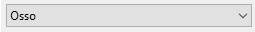
\includegraphics[scale=0.65]{../user_guide_figures/invesalius_screen/segmentation_threshold_presets_pt.png}
\caption{Caixa de seleção de valores pré-definidos de limiar}
\label{fig:limiar_presets}
\end{figure}

A tabela \ref{tab:limiar} mostra a faixa de níveis de cinza de acordo com o tipo de tecido ou material.

\begin{table}[h]
\centering
\caption{Limiares pré-definidos para alguns materiais}
\begin{tabular}{lcc}\\
\hline % este comando coloca uma linha na tabela
Material & Limiar inicial & Limiar final\\
\hline
\hline
Esmalte (Adulto) & 1553 & 2850\\
Esmalte (Criança) & 2042 & 3021\\
Osso & 226 & 3021\\
Osso Compacto (Adulto) & 662 & 1988\\
Osso Compacto (Criança) & 586 & 2198\\
Osso Esponjoso (Adulto) & 148 & 661\\
Osso Esponjoso (Criança) & 156 & 585\\
Personalizado & Def. Usuário & Def. Usuário\\
Tecido Epitelial (Adulto) & -718 & -177\\
Tecido Epitelial (Criança) & -766 & -202\\
Tecido Gorduroso (Adulto) & -205 & -51\\
Tecido Gorduroso (Criança) & -212 & -72\\
Tecido Muscular (Adulto) & -5 & 135\\
Tecido Muscular (Criança) & -25 & 139\\
Tecidos Moles & -700 & 225\\
\hline
\end{tabular}
\label{tab:limiar}
\end{table} 
\newpage

A tabela \ref{tab:limiar} é mais indicada para tomógrafos médicos. Nos tomógrafos odontológicos,
comumente as faixas de níveis de cinza são maiores e não regulares. Assim, é necessário utilizar
a barra de limiar (figura \ref{fig:region_selection_bar}) para ajustá-las.

Caso se deseje criar uma nova máscara, basta clicar no ícone do atalho presente no painel, dentro
do item \textbf{2. Selecione a região de interesse}. Veja a figura \ref{fig:shortcut_new_mask}.

\begin{figure}[!htb]
\centering

\includegraphics[scale=0.2]{../user_guide_figures/icons/object_add_original.png}
\caption{Atalho para criar nova máscara}
\label{fig:shortcut_new_mask}
\end{figure}

Clicando-se nesse atalho, uma nova janela será apresentada (figura \ref{fig:create_new_mask}).
Selecione a faixa de limiar desejada e clique em \textbf{OK}.

\begin{figure}[!htb]
\centering
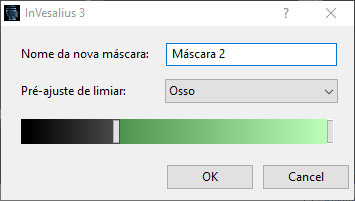
\includegraphics[scale=0.55]{../user_guide_figures/invesalius_screen/segmentation_threshold_window_dialog_pt.png}
\caption{Criar uma nova máscara}
\label{fig:create_new_mask}
\end{figure}

\newpage

Com uma máscara de segmentação configurada, é possível gerar a superfície 3D correspondente
às imagens em estudo. A superfície será composta por uma malha de triângulos. O próximo capítulo
trará maiores detalhes sobre esse tipo de superfície.

Para iniciar a geração, clique no botão \textbf{Gerar superfície} (figura \ref{fig:generate_surface}).
Caso já exista uma superfície gerada previamente, pode-se substituí-la pela nova. Para isso, basta
selecionar, \textbf{antes} da geração, a opção \textbf{Sobrescrever anterior}.

\begin{figure}[!htb]
\centering
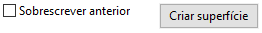
\includegraphics[scale=0.55]{../user_guide_figures/invesalius_screen/segmentation_generate_surface_pt.png}
\caption{Botão Gerar superfície}
\label{fig:generate_surface}
\end{figure}

Após alguns instantes, a superfície será exibida na janela de visualização 3D do InVesalius
(figura \ref{fig:surface}).

\begin{figure}[!htb]
\centering
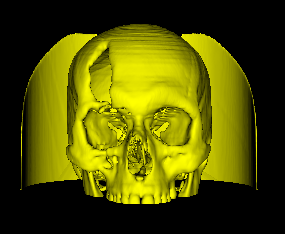
\includegraphics[scale=0.5]{../user_guide_figures/invesalius_screen/surface_from_threshold.png}
\caption{Superfície 3D}
\label{fig:surface}
\end{figure}
 


\section{Segmentação manual (Edição de imagens)}

Há situações em que a segmentação por limiar não é eficiente, pois ela é aplicada ao conjunto
todo das imagens. Para aplicar a segmentação a imagens isoladas, pode-se usar a segmentação
manual. Com ela, é possível adicionar ou apagar uma determinada região da imagem que foi
segmentada por limiar. No entanto, a segmentação manual requer maior conhecimento de anatomia
por parte do usuário. Para utilizá-la, é necessário clicar em \textbf{Edição Manual} (figura \ref{fig:advanced_edition}) para abrir o painel de edição.

\begin{figure}[!htb]
\centering

\includegraphics[scale=0.75]{../user_guide_figures/invesalius_screen/segmentation_manual_label_pt.png}
\caption{Ícone para abrir a ferramenta de edição manual}
\label{fig:advanced_edition}
\end{figure}

O painel de edição aparece como mostra a figura \ref{fig:edition_slices_ref}.

\begin{figure}[!htb]
\centering
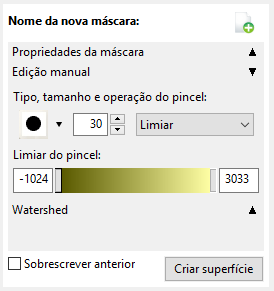
\includegraphics[scale=0.6]{../user_guide_figures/invesalius_screen/segmentation_manual_window_pt.png}
\caption{Painel de edição}
\label{fig:edition_slices_ref}
\end{figure}

Há dois tipos de pincel disponíveis para desenho: um em forma de círculo e outro em forma
de quadrado. Para escolher um pincel, clique no triângulo da lista de seleção para abri-la
e, a seguir, clique sobre o tipo escolhido. O pincel selecionado aparece no painel como
mostra a figura \ref{fig:brush_type}.

\begin{figure}[!htb]
\centering
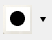
\includegraphics[scale=0.9]{../user_guide_figures/invesalius_screen/segmentation_manual_pencil_type.png}
\caption{Tipo de pincel}
\label{fig:brush_type}
\end{figure}

\newpage

Também é possível alterar o diâmetro do pincel, conforme mostra a figura \ref{fig:select_diameter}.

\begin{figure}[!htb]
\centering
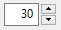
\includegraphics[scale=0.8]{../user_guide_figures/invesalius_screen/segmentation_manual_diameter.png}
\caption{Seleção do diâmetro do pincel}
\label{fig:select_diameter}
\end{figure}

É necessário selecionar o tipo de operação que será realizada pelo pincel. As opções são as
seguintes:

\begin{itemize}
	\item \textbf{Desenhar}, para pintar uma região que não foi selecionada;
	\item \textbf{Apagar}, para remover uma região que foi selecionada;
	\item \textbf{Limiar}, para remover uma região que está fora do limiar e foi selecionada, ou pintar
uma região que está dentro do limiar e não foi selecionada.
\end{itemize}

A figura \ref{fig:select_brush_operations} ilustra a lista de operações do pincel:

\begin{figure}[!htb]
\centering
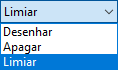
\includegraphics[scale=0.7]{../user_guide_figures/invesalius_screen/segmentation_manual_pencil_type_operation_type_pt.png}
\caption{Seleção do tipo de operação do pincel}
\label{fig:select_brush_operations}
\end{figure}

A figura \ref{fig:noise_amalgaman} mostra um caso em que algumas imagens contêm ruídos
causados pela presença de prótese dentária de amálgama no paciente. Observe os "raios" 
saindo da região da arcada dentária. Isso ocorre porque a máscara de segmentação também
seleciona parte dos ruídos, pois eles estão na mesma intensidade do limiar para osso.

\begin{figure}[!htb]
\centering
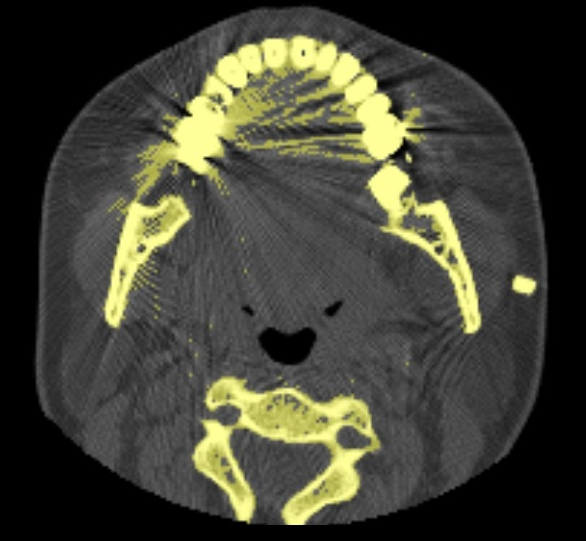
\includegraphics[scale=0.3]{../user_guide_figures/invesalius_screen/segmentation_manual_noise_amalgam.jpg}
\caption{Imagem com ruído segmentada com limiar}
\label{fig:noise_amalgaman}
\end{figure}

A figura \ref{fig:surface_amagaman} ilustra como é uma superfície gerada a partir dessa
segmentação.

\begin{figure}[!htb]
\centering
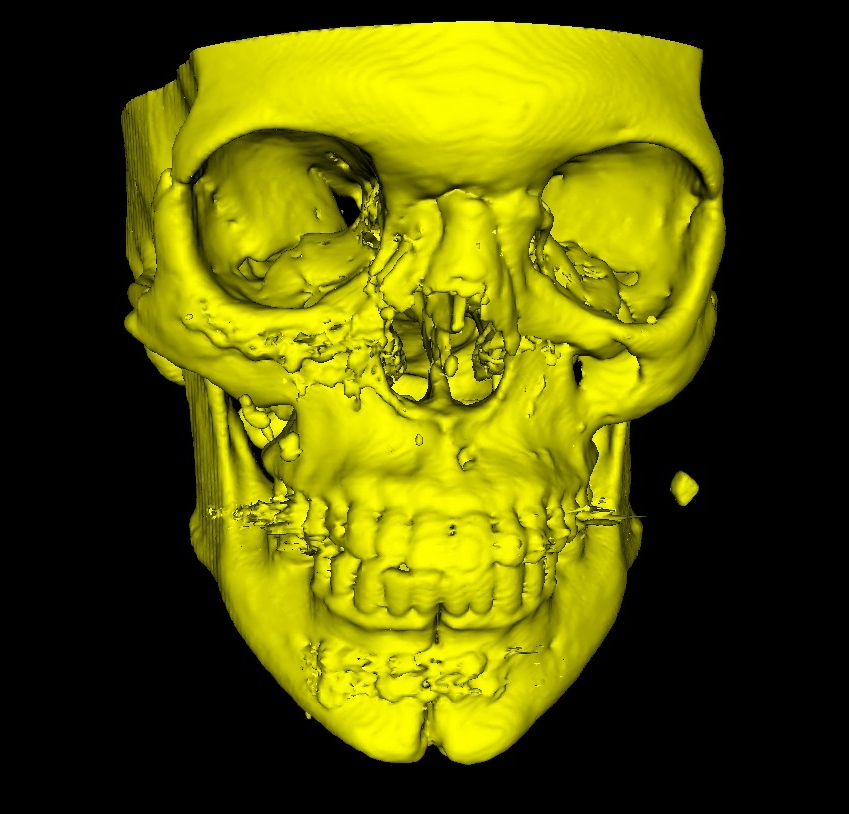
\includegraphics[scale=0.3]{../user_guide_figures/invesalius_screen/segmentation_manual_noise_amalgam_3d.jpg}
\caption{Superfície gerada a partir de imagem com ruído}
\label{fig:surface_amagaman}
\end{figure}

\begin{figure}[!htb]
\centering
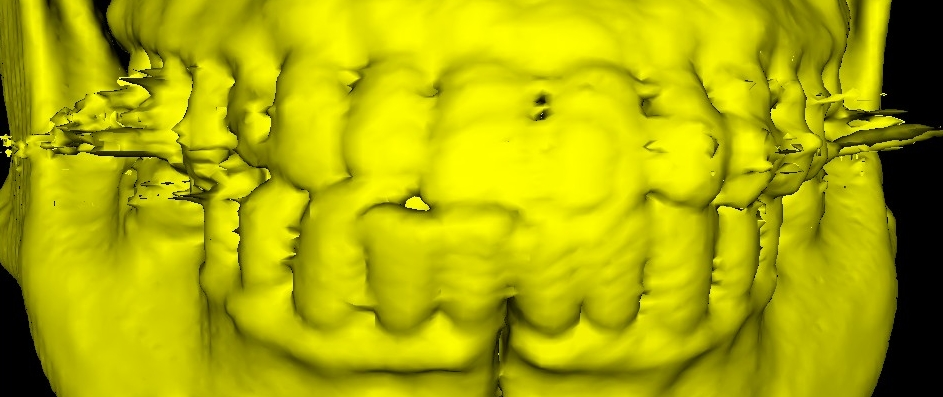
\includegraphics[scale=0.3]{../user_guide_figures/invesalius_screen/segmentation_manual_noise_amalgam_3d_zoom.jpg}
\caption{Zoom da região com ruído}
\label{fig:surface_amagaman_zoom}
\end{figure}

\newpage

Em casos como este, utilizando o editor, com o pincel na opção \textbf{Apagar}, mantenha o
botão \textbf{esquerdo} do mouse pressionado enquanto o \textbf{arrasta} sobre a região que
deseja remover (na máscara).

A figura \ref{fig:editor_amalgaman} mostra a imagem da figura \ref{fig:noise_amalgaman} após
edição.

\begin{figure}[!htb]
\centering
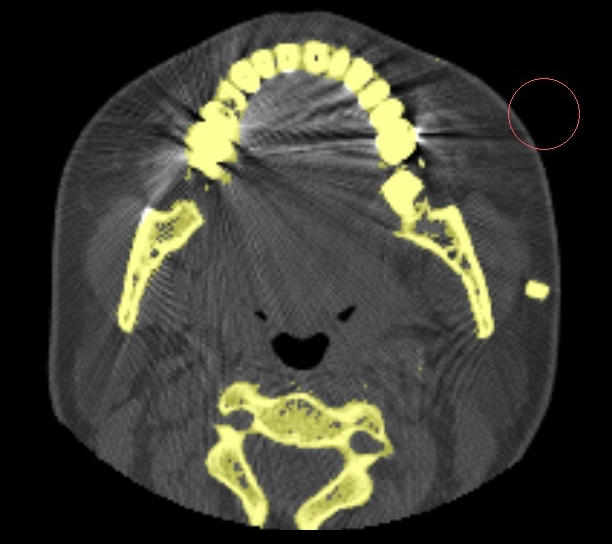
\includegraphics[scale=0.3]{../user_guide_figures/invesalius_screen/segmentation_manual_noise_amalgam_removed.jpg}
\caption{Imagem com ruído removido}
\label{fig:editor_amalgaman}
\end{figure}

\begin{figure}[!htb]
\centering
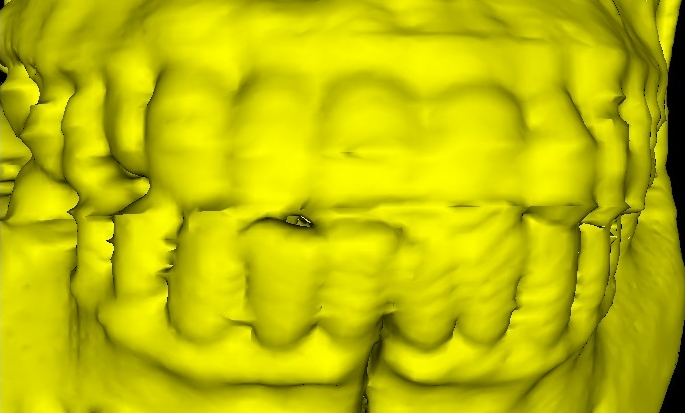
\includegraphics[scale=0.3]{../user_guide_figures/invesalius_screen/segmentation_manual_noise_amalgam_removed_3d_zoom.jpg}
\caption{Superfície criada a partir da imagem com ruído removido}
\label{fig:surface_edited_amalgaman}
\end{figure}

\newpage
Realizada a edição, basta gerar a superfície a partir da imagem editada (figura
\ref{fig:surface_edited_amalgaman}). Como houve edição, ao clicar em \textbf{Criar superfície}, será
requerido se deseja gerar a superfície a partir do método \textbf{binário} ou utilizando o método de suavização
\textbf{Suavização sensível ao contexto} (figura \ref{fig:new_surface_edited}) para minimizar os "degraus" na superfície.
Demais detalhes serão discutidos no capítulo \ref{cap_surface}.
%\ref{fig:generate_surface}).

\begin{figure}[!htb]
\centering
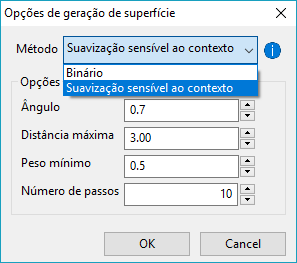
\includegraphics[scale=0.5]{../user_guide_figures/invesalius_screen/surface_generation_dialog_pt.png}
\caption{Método de criação de superfície}
\label{fig:new_surface_edited}
\end{figure}


\section{Watershed}

A segmentação por watershed, necessita que o usuário indique através de marcadores o que é objeto e o que é fundo. Esse método de segmentação interpreta a imagem como uma bacia hidrográfica, sendo que os valores dos níveis de cinza são as altitudes, formando vales e montanhas, os marcadores de fundo e objeto são as fontes de água. Essas fontes de água, começam "encher" essa bacia hidrográfica até se encontrarem, assim segmentando a imagem em fundo e objeto. Para utilizá-la, é necessário clicar na opção \textbf{Watershed} para abrir o painel de edição (figura~\ref{fig:watershed_painel}).

\begin{figure}[!htb]
\centering
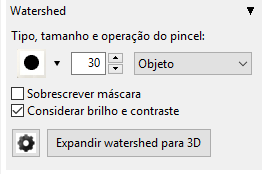
\includegraphics[scale=0.75]{../user_guide_figures/invesalius_screen/segmentation_watershed_panel_pt.png}
\caption{Painel de segmentação por Watershed}
\label{fig:watershed_painel}
\end{figure}

Antes de iniciar a segmentação por Watershed, é recomendável limpar toda a máscara utilizando a ferramenta de limpeza de máscara, conforme é mostrado na seção~\ref{cap:limpeza_mascara}.

Para inserir marcadores de fundo e objeto, é utilizada uma ferramenta em forma de pincel, a exemplo da segmentação manual, existe a opção de selecionar pincel retangular ou circular, também é possível alterar o tamanho deles. 

É necessário também selecionar o tipo de operação que será realizada pelo pincel. As opções são as
seguintes:
\begin{itemize}
\item \textbf{Objeto}, para inserir marcadores de objeto;
\item \textbf{Fundo}, para inserir marcadores de fundo (não é objeto);
\item \textbf{Apagar}, para apagar marcadores de objeto ou fundo.
\end{itemize}

A opção "\textbf{Sobrescrever máscara}" é utilizada quando deseja-se que a máscara selecionada seja substituída pelo resultado da segmentação. Já a opção "\textbf{Considerar brilho e contraste}" é utilizada para o algoritmo levar em consideração a imagem que está sendo visualizada, assim é possível alterar o brilho e contraste e obter resultados melhores de segmentação.

É possível configurar o método de \textit{Watershed} através do botão ao lado esquerdo do painel (figura~\ref{fig:watershed_conf}). Ao abrir essa opção é mostrada a janela~\ref{fig:watershed_janela_conf}. A opção método permite alterar o algoritmo que é utilizado na segmentação, existe o Wartershed convencional e o Watershed baseado no método de IFT (\textit{Image Forest Transform}), em alguns casos, como segmentação de cérebro ele apresenta melhor resultado.

A conectividade dos pixels que serão levados em consideração, pode ser alterados, no caso 2D, é possível selecionar conectividade $4$ e $8$, já no caso 3D pode-se selecionar $6$,$18$ ou $26$. O valor "\textbf{Sigma da gaussiana}" é alterado para o método suavizar mais ou menos a imagem ao aplicar a segmentação, valores altos tendem a deixar a imagem mais suavizada e consequentemente o algoritmo seleciona menos detalhes e ruídos.

\begin{figure}[!htb]
\centering

\includegraphics[scale=0.5]{../user_guide_figures/icons/configuration.png}
\caption{Botão para abrir a configuração do método de Watershed}
\label{fig:watershed_conf}
\end{figure}

\begin{figure}[!htb]
\centering
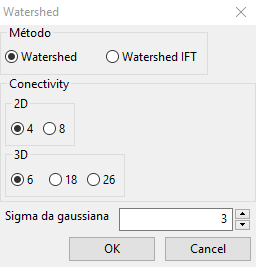
\includegraphics[scale=0.55]{../user_guide_figures/invesalius_screen/segmentation_watershed_conf_pt.png}
\caption{Opções de configuração do método de Watershed}
\label{fig:watershed_janela_conf}
\end{figure}

Existe a opção do método ser executado para todo o volume (expandir para outras fatias), para isso, após ser inserido os marcadores de objeto e de fundo, é necessário clicar no botão \textbf{Expandir watershed para 3D}, localizado no painel. Na figura~\ref{fig:watershed_2d} é exibido o resultado da segmentação do cérebro em uma fatia (2D), já na figura~\ref{fig:watershed_3d} é mostrado a expansão para todo o volume (3D). 

Ainda na figura~\ref{fig:watershed_2d}, podemos visualizar os marcadores de objeto em verde claro, os marcadores de fundo em vermelho e a máscara em verde transparente cobrindo a região selecionada (resultado).

\begin{figure}[!htb]
\centering
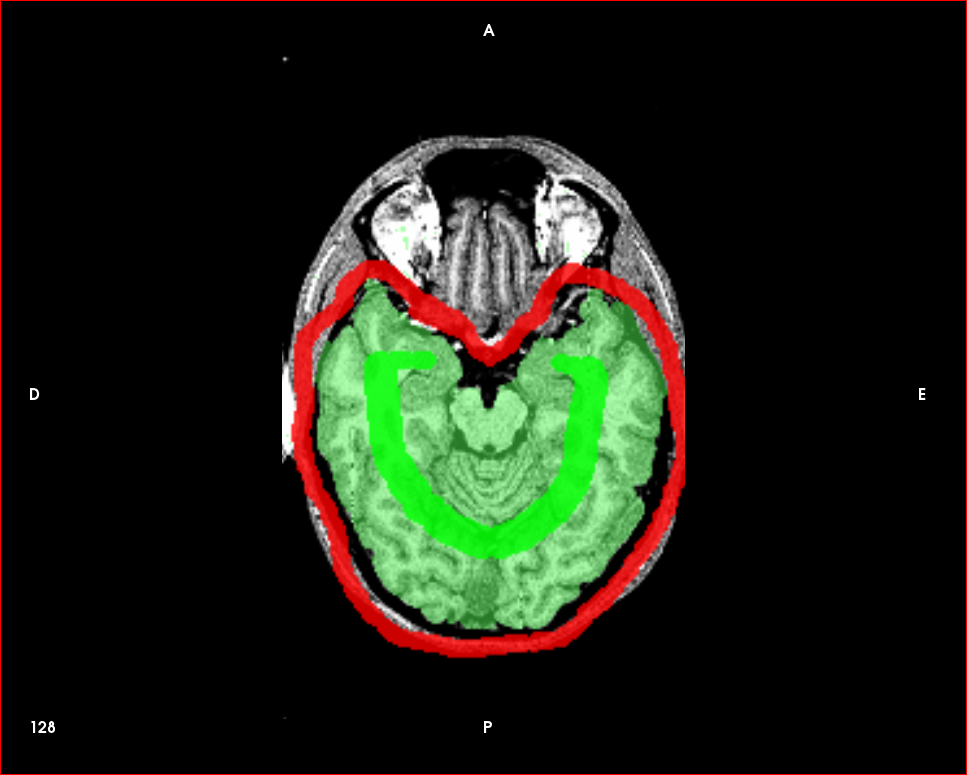
\includegraphics[scale=0.2]{../user_guide_figures/invesalius_screen/segmentation_watershed_axial.png}
\caption{Watershed aplicado em uma fatia de um volume.}
\label{fig:watershed_2d}
\end{figure}

\begin{figure}[!htb]
\centering
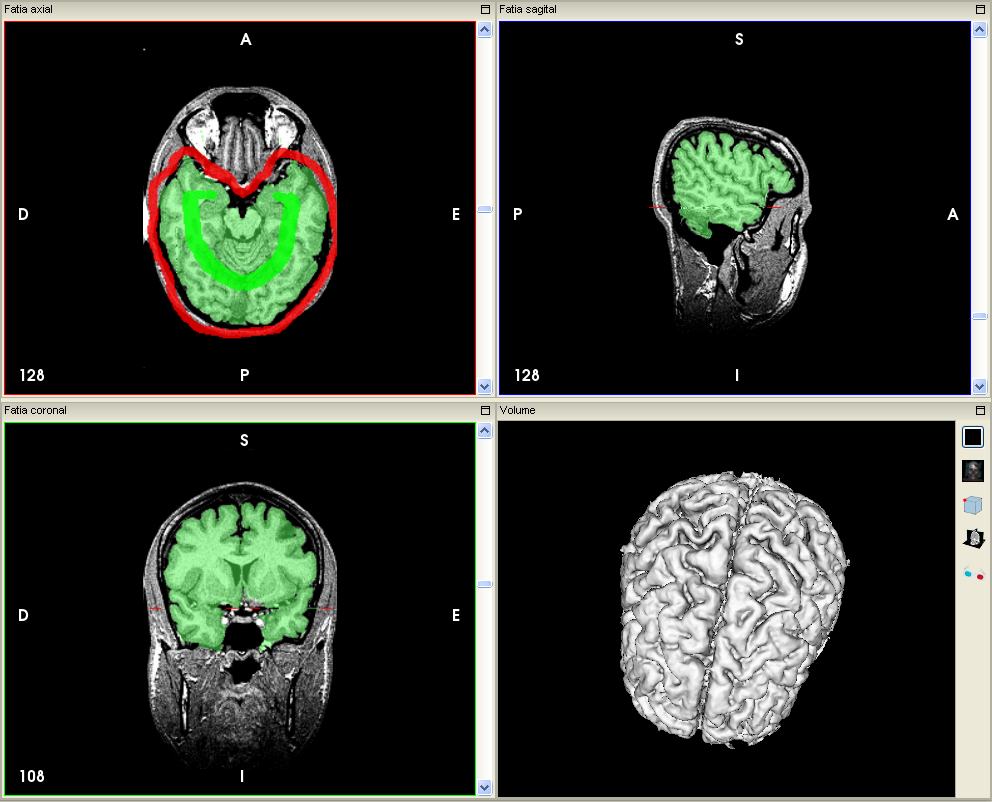
\includegraphics[scale=0.4]{../user_guide_figures/invesalius_screen/segmentation_watershed_multiplanar_3d_pt.png}
\caption{Segmentação do cérebro com o método de Watershed aplicado em todo um volume (expandido em 3D).}
\label{fig:watershed_3d}
\end{figure}

\section{Crescimento de região}

A técnica de segmentação por crescimento de região é ativada no menu \textbf{Ferramentas}, \textbf{Segmentação}, por último \textbf{Crescimento de região} (figura~\ref{fig:menu_segmentation_region_growing}). Inicialmente deve-se selecionar a configuração entre \textbf{2D - Fatia atual} ou \textbf{3D - Todas as fatias}, também é necessário selecionar a conectividade do crescimento entre $4$ ou $8$ para o 2D e $6$, $18$ ou $26$ para 3D. Por último é necessário selecionar o método, entre \textbf{Dinâmico, Limiar ou Confidência} (figura~\ref{fig:segmentation_region_growing_dinamic}).

\begin{figure}[!htb]
\centering
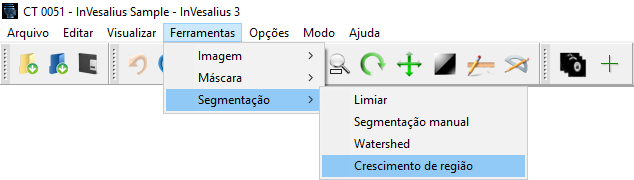
\includegraphics[scale=0.5]{../user_guide_figures/invesalius_screen/menu_segmentation_region_growing_pt.png}
\caption{Menu para ativar a segmentação por região de crescimento.}
\label{fig:menu_segmentation_region_growing}
\end{figure}

\begin{figure}[!htb]
\centering
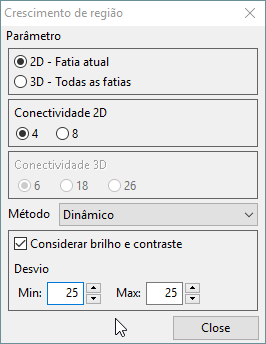
\includegraphics[scale=0.7]{../user_guide_figures/invesalius_screen/segmentation_region_growing_dinamic_pt.png}
\caption{Tela para ajuste de parâmetros de segmentação por crescimento de região.}
\label{fig:segmentation_region_growing_dinamic}
\end{figure}

A técnica parte de um pixel inicial que é indicado clicando com o \textbf{botão esquerdo} do mouse, os pixels vizinhos que satisfazem as condições indicadas anteriormente são selecionados. Cada método leva em consideração diferentes condições, a seguir são apresentadas as diferenças entre cada método:

\begin{itemize}
	\item \textbf{Dinâmico}: Esse método captura o valor do pixel que foi clicado, levando em consideração o desvio para baixo (min) e desvio para cima (max). A opção \textbf{Considerar o brilho e contraste} é ativada por padrão, essa opção permite levar em consideração os valores de níveis de cinza que são exibidos e/ou ajustados na opção brilho e contraste. Ao desativar essa opção será levado em consideração os valores de cinza gravados na imagem (figura~\ref{fig:segmentation_region_growing_dinamic_parameter}). 
	
	\begin{figure}[!htb]
	\centering
	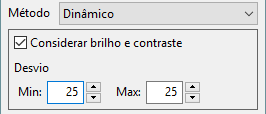
\includegraphics[scale=0.7]{../user_guide_figures/invesalius_screen/segmentation_region_growing_dinamic_parameter_pt.png}
	\caption{Ajuste de parâmetros para o método dinâmico.}
	\label{fig:segmentation_region_growing_dinamic_parameter}
	\end{figure}
	
	\item \textbf{Limiar}: O método limiar selecionará os pixels cuja a vizinhança estejam dentro do valor mínimo e máximo (figura~\ref{fig:segmentation_region_growing_limiar}).

	\begin{figure}[!htb]
	\centering
	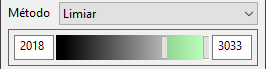
\includegraphics[scale=0.7]{../user_guide_figures/invesalius_screen/segmentation_region_growing_limiar_pt.png}
	\caption{Ajuste de faixa de valores do método limiar.}
	\label{fig:segmentation_region_growing_limiar}
	\end{figure}	
	
\item \textbf{Confidência}: Esse método inicia calculando o desvio padrão e a média do pixel selecionado pelo usuário e sua vizinhança. Pixels conectados com valores dentro da faixa (que é dado pela média mais e menos o desvio padrão multiplicado pelo \textbf{multiplicador}). É calculada a média e desvio padrão dos pixeis selecionado. Que é seguido por outra etapa de expansão. Esse processo é repetido de acordo com o parâmetro \textbf{Iteração}. A figura~\ref{fig:segmentation_region_growing_confidence_parameter} mostra os parâmetros desse método.
	
	\begin{figure}[!htb]
	\centering
	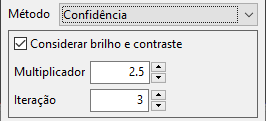
\includegraphics[scale=0.7]{../user_guide_figures/invesalius_screen/segmentation_region_growing_confidence_parameter_pt.png}
	\caption{Ajuste de faixa de valores do método limiar.}
	\label{fig:segmentation_region_growing_confidence_parameter}
	\end{figure}	
	
	
\end{itemize}
